\documentclass[a4paper,12pt]{article}
\usepackage{geometry}
\geometry{left=2.54cm,right=2.54cm,top=2.54cm,bottom=2.54cm}
\usepackage{amsmath}
\usepackage{amsfonts}
\usepackage{graphicx}
\usepackage{bbm}
\usepackage{pifont}
\usepackage{indentfirst}
\usepackage{wrapfig}
\usepackage{color}
\usepackage{enumerate}
\usepackage{amssymb, graphics, setspace}
\usepackage{url}
\usepackage{float}

\begin{document}
	
	\vspace*{0.25cm}
	\begin{center}
		
\includegraphics[scale=0.9]{LOGO.png}
	\end{center}
	
	\thispagestyle{empty}
	
	\begin{center}
		
		\hrulefill
		
		\vspace*{5cm}
		\begin{Huge}
			\sc{VE572 \\Methods and tools
				for big data\\[0.6em]
				Lab 1 Report}
		\end{Huge}
		
		\vspace{1em}

	\end{center}
	
	\vfill
	
	\begin{center}
		\begin{align*}			
		\text{Lin Zhi } & \quad 5143709113\\[0.5em]
		\text{Liu Yihao } & \quad 515370910207\\[0.5em]
		\text{Zhou Yanjun } & \quad515370910219\\[0.5em]
		\text{Zhou Zhuangzhuang } & \quad 5143709184
		\end{align*}
	\end{center}
	\vspace*{3cm}
	\begin{center}
		28 May 2018 
	\end{center}
	
	\newpage
	\newgeometry{left=3.18cm,right=3.18cm}
	
	
	\section{Server Access}
	The IP address of the server is 45.76.213.89. User can use the two private SSH key to login the server as administrative account.
	
	\section{Documentation}
	\subsection{TCPServer}
	\noindent\textbf{Functions \& Classes in TCPServer.java}
	
	\noindent\textbf{public static void main(String[] args)} Listen the socket request from clients through port 7650 and create a new Handler to solve each command from clients. 
	
	\noindent\textbf{public static class Handler} A class extending Threads. It has functions as follows:
	\begin{enumerate}
		\item \textbf{Handler(Socket socket, int clientNumber)} Constructor.
		\item \textbf{public void run()} Read commands from socket, call functions to deal with the command and close socket after the command finished.
		\item \textbf{private boolean readLine(BufferedReader input, PrintWriter output)} Parse the commands and check whether a command has finished.
		\item \textbf{private boolean runCommand(String[] args, PrintWriter output)} Check whether the commands are in the right order and format and deal with the correct commands by calling other functions.
		\item \textbf{private String saveFile(int size, String type)} Get the input stream from the socket and save it as the file with a name consisted of date and hash string and the corresponding type. 
		\item \textbf{private void log(String message)} Print information for the server end.
	\end{enumerate}
	
	\subsection{DataExtractor}
	\noindent\textbf{Functions \& Classes in DataExtractor.java}
	
	\noindent\textbf{public class DataExtractor}
	\begin{enumerate}
		\item \textbf{public DataExtractor(String Filename)} Constructor.
		\item \textbf{private class MeaQuantity} A class storing informatin for a measure quantity.
		\begin{enumerate}
			\item \textbf{private void parseShort(ByteBuffer buffer)} Read short type data from ByteBuffer, store them in a private Number variable data and sum them up. We also provide parseLong for Integer, parseFloat for Float and parseDouble for Double.
			\item \textbf{private Number[] calculate()} Sort and find min and max for data.
			\item \textbf{private void calculateShort()} Call calculate() and find the median and average of the data. We also provide calculateLong for Integer, calculateFloat for Float and calculateDouble for Double.
		\end{enumerate}
		\item \textbf{public void parse()} Extract and save the data from the XML file, including the Name, DataType, Quantity and Unit. The Quantity and Unit are first recorded as Id from MeaQuantity Node and then checked the Quantity Node or Unit Node to find the Name of them.
		\item \textbf{public String query(String name, String op)} Check the Option from the command, search the min, max, median, sum or average of the measure quantity and format the output string.
		\item \textbf{public void readBinary(String fileName)} Read the binary file and parse the data with the corresponding data type.
		\item \textbf{public void writeXlsx(String fileName)} Write the quantities' name, unit and data in binary file into an excel file with poi package.
	\end{enumerate}
	
	
	\section{Progress}
	\noindent\textbf{I. Own a remote server on a public cloud platform}
	
	We have set up a remote server at IP address 45.76.213.89 and upload the programs on it. Users can login the server as root account with their private keys.  
	
	\noindent\textbf{II. Implement a socket protocol in Java}
	
	In TCPServer.java, we implement the socket protocol with the ServerSocket and Socket package. The server can recieve commands from the client with socket protocol. The commands can be dealt with are
	
		1. BEGIN;
		
		2. SIZE Type Size; Type is one of XML or BIN
		
		3. QUERY Op Name; Op is one of MAX, MIN, AVG, SUM, and MEDIAN.
		
		4. END;

	We expect the commands are in the following order: BEGIN, SIZE XML, SIZE BIN, a certain number of QUERY, and END. If the command is not in such an order, the sever will report "Error: command unexpected". If an unexpected Op is receieved, the server will report ""Error: Op not available". Message "OK" will be sent to client for each valid command and query result will be showed for QUERY command.
	
	The corresponding BIN or XML file sent by client will be saved on the server. The file name is comprised by the date and a hash string to make sure its uniqueness. 
	
	 
	\noindent\textbf{III. Write a Java program to extract data from an XML file}
	
	In DataExtractor.java, we use external package dom4j to extract information from XML file. The recorded information includes Name, Unit, Quantity and the location like the startOffset, blocksize and valueOffset of the corresponding data in the BIN file. 
	
	
	\noindent\textbf{IV. Dump the data from a binary file}
	With the information extracted from the XML file, we locate the data for each measure quantity in the binary file, read it in little endian and save it. At the same time, we calculate the MAX, MIN, AVG, SUM, and MEDIAN for each measure quantity so that it can be used for the QUERY commands.
	
	We also use external package poi to save the data from the binary file along with the name and unit of the measure quantities into an XLSX file.
	
	\noindent\textbf{V. Complete all the tasks into a remote server application}
	
	All the source files including a sample client are uploaded into the server. Users can compile and run the programs according to the following commands:
	
	\textbf{Install} 
	
	mvn install
	
	\textbf{Run the server} 
	
	mvn exec:java -Dexec.mainClass="TCPServer"
	
	\textbf{Run the client} 
	
	mvn exec:java -Dexec.mainClass="TCPClient" -Dexec.args="$ < $host$ > $"
	
	These commands can also be found in the README.md on the server.
	
	\section{Main Discoveries}
	Here are the main discoveries during the lab:
	\begin{enumerate}
		\item When setting up a socket connectiong, we learn that the server needs new threads to deal with the new commands. To do that, we define a class extending Thread to handle each command from client. 
		\item When extracting data from the XML file, we find a useful external library dom4j. 
		\item When reading data from the BIN file, we discover a convienient data type named ByteBuffer which can be set to read data as little endian and has functions to get variables in different data types. 
	\end{enumerate}
	
	
	
	\section{Attempts And Failures}
	We attempt to read the binary file directly but notice that the result gives a number like "-6.5798...E307". The number seems so strange that we recheck the process and find that in Java the default I/O stream is big endian while it might be little endian for the binary file. Then we read the binary file in little endian and comfirm that it is right with the given decoding set of files. 
	
	We once confused about why for the same data type ieeefloat8, we have blocksize with both 8 and 18 in the validate.xml file. After more considerations, we realize that it might be a struct contained several different data type. And we successfully find another ieeefloat8 type and a dt\_short type with blocksize of 18.  
	
	\section{Self-evaluation}
	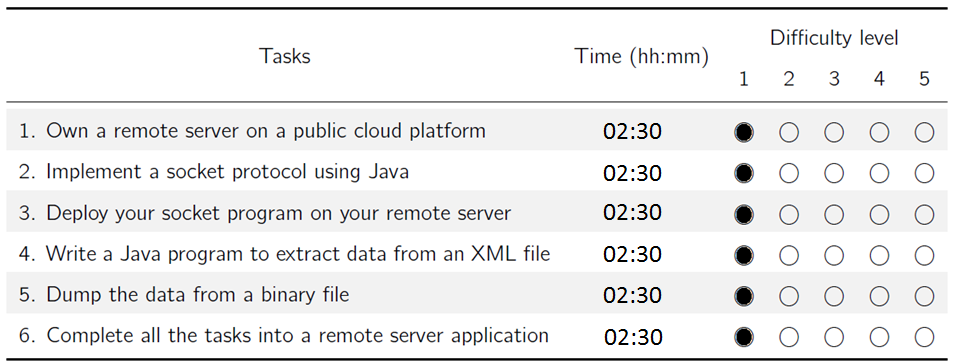
\includegraphics[scale = 0.7]{evaluation}
	

\end{document}